\chapter{Frontend}\label{ch:B}

\section{Stack of technologies}
    \subsection{Typescript}
    JavaScript is a dynamic typing language, which means that type of the variable can be changed and will be defined by assigned value. Is it always suitable? Surely, no. Sometimes we need to know which exactly type is a variable, cause our application could crash, if we don't receive proper field or field format. Typescript can help us to prevent this type of issues, cause it's a static typing language. So we can't assign value with type B to the variable once we've assigned value with type A to it. Also Typescript has such features like the Generic types, Declaration files etc.
    \subsection{React}
    React is a JavaScript library. It's a one of the most popular JavaScript frameworks(libraries) for building user interfaces. It's free and open-source, which means that everyone can contribute to it. Developing in React based on UI components. React code is easy to understanding, because of JSX(JavaScript Syntax Extension). JSX allows you to assign html elements to the variables and write JavaScript code inside of html code. React has a Virtual DOM, which provides fast changes in DOM tree with reconciliation.
    Also notable features of React: declarative, lifecycle methods, hooks, state and props.
    
    \subsection{Redux}
    Redux is a state management tool for React based on flux architecture. 
    \\\\Redux flow:
    \\1. UI (User Interface)
    \\2. Actions
    \\3. Reducer
    \\4. Store
    \\5. State
    \subsection{Material-UI}
    Material UI is a tool which provides scalable UI components for React.
    \subsection{Axios}
    Axios is a tool for easily making a request for server.
    \subsection{react-router-dom}
    react-router-dom is a library for configure pages routing in react app.
    \subsection{SCSS}
    SCSS is a tool which help to work with styles easier.

\section{Maze game implementation}
    \subsection{Throttling}
    To throttle a function means to ensure that the function is called at most once in a specified time period (for instance, once every 10 seconds). This means throttling will prevent a function from running if it has run “recently”. Throttling also ensures a function is run regularly at a fixed rate.
    \\\\Simple example of throttle function:
    \begin{lstlisting}
        export function throttle(callback, interval) {
            let enableCall = true;
          
            return function(...args) {
              if (!enableCall) return;
          
              enableCall = false;
              console.log(args)
              callback.apply(this, args);
              setTimeout(() => enableCall = true, interval);
            }
        }
		\end{lstlisting}


    \begin{figure}
      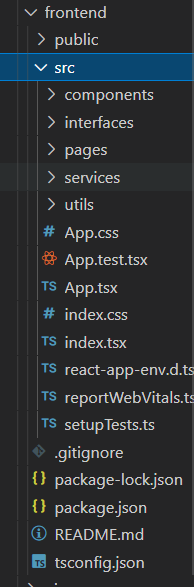
\includegraphics[width=0.4\linewidth]{structure.png}
      \caption{The project structure}
      \label{fig:structure}
    \end{figure}
    \begin{figure}
      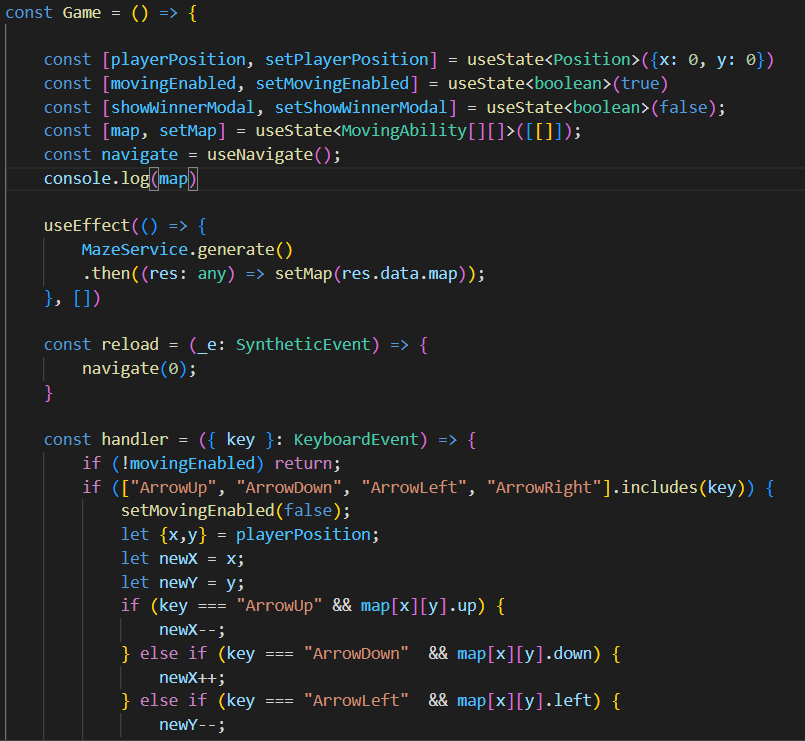
\includegraphics[width=\linewidth]{game-page.png}
      \caption{GamePage component}
      \label{fig:game-page}
    \end{figure}